\section{Расчетно-конструкторская часть}
%    \subsection{Описание базовой системы стенда исследования упругих колебаний %
%        в двухмассовой системе электропривода}
        
        Лабораторно исследовательский стенд  представляет собой
        электромеханическую систему на базе асинхронного двигателя с
        короткозамкнутым ротором (рисунок \ref{fig:general-view}).

        \begin{figure}[h!]
            \center{
                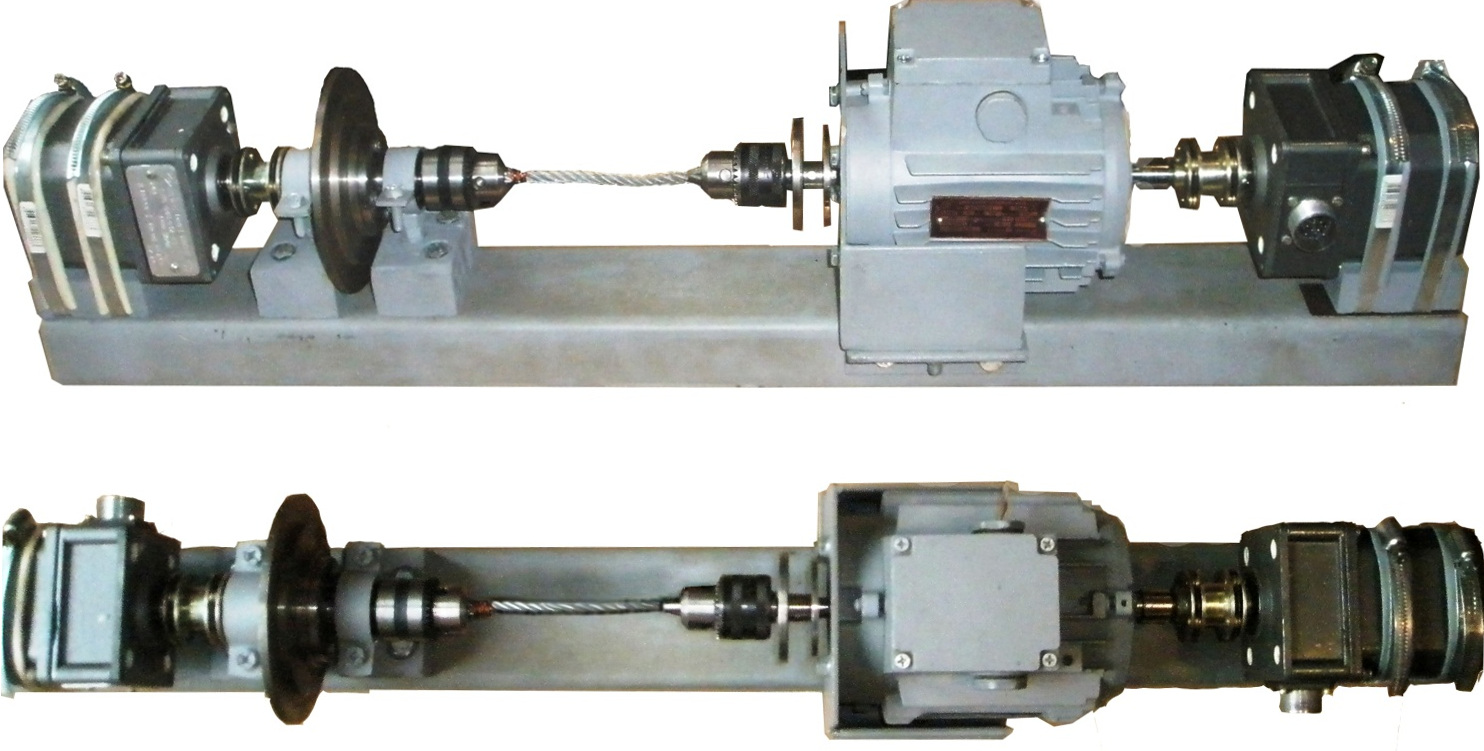
\includegraphics[width=0.8\linewidth]{img/general-view}
            }
            \caption{Общий вид лабораторно исследовательского стенда}
            \label{fig:general-view}
        \end{figure}
        
        В состав стенда входит:
        \begin{itemize}
            \item асинхронный двигатель АИР56А4У3;
            \item 2 фотоэлектрических дискретных датчика перемещения ПДФ-5 с
            разрешающей способностью  600 имп/об;
            \item упругий вал;
            \item силовой блок автономного инвертора напряжения;
            \item блок управления автономным инвертором напряжения.
        \end{itemize}

        Система управления обеспечивает плавный пуск и останов асинхронного
        электродвигателя, с возможностью регулировки частоты вращения. Так же
        система обеспечивает связь с ПК для мониторинга и контроля основных
        параметров.
          
        Питание системы осуществляется от бытовой сети 220 В переменного тока.

    \subsection{Структурная схема системы управления электропривода
        лабораторно - исследовательского стенда}

        Структурная схема системы управления электроприводомлабораторно
        исследовательского стенда представлена на рисунке \ref{fig:struct}.

        \begin{figure}[h!]
            \center{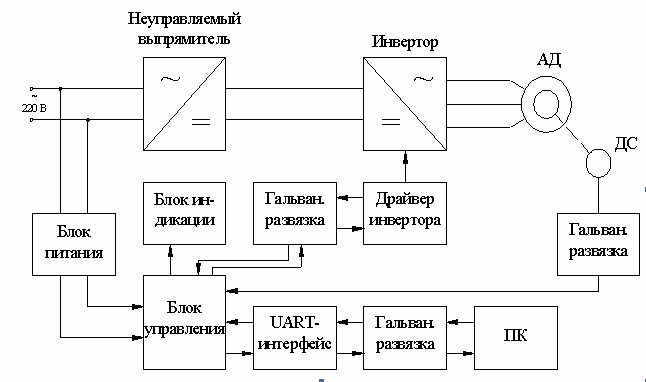
\includegraphics[width=1.0\linewidth]{img/struct}}
            \caption{Структурная схема лабораторно исследовательского стенда}
            \label{fig:struct}
        \end{figure}

        Система частотного электропривода стенда построена по схеме
        двойного преобразования.  Она состит из следующих основных частей:
        звена  постоянного  тока  (неуправляемого выпрямителя), силового
        импульсного инвертора и блока управления.

        Звено постоянного тока состоит из неуправляемого выпрямителя и фильтра.
        Переменное напряжение питающей сети преобразуется в нем в напряжение
        постоянного тока.

        Силовой трехфазный импульсный инвертор состоит из шести транзисторных
        ключей. Каждая обмотка электродвигателя подключается через
        соответствующий ключ к положительному и отрицательному выводам
        выпрямителя. Инвертор осуществляет преобразование выпрямленного
        напряжения в трехфазное переменное напряжение нужной частоты и амплитуды,
        которое прикладывается к обмоткам статора электродвигателя.

        В выходных каскадах инвертора в качестве ключей используются силовые
        MOSFET-транзисторы. По сравнению с тиристорами они имеют более высокую
        частоту переключения, что позволяет вырабатывать выходной сигнал
        синусоидальной формы с минимальными искажениями. 

        Блок управления формирует ШИМ сигналы управления силовым модулем
        инвертора напряжения. В управляющем микроконтроллере блока управления
        програмно реализован алгоритм скалярного управления частотой
        асинхронного двигателя по принципу постоянства отношения напряжения на
        обмотках статора двигателя к частоте этого напряжения (закон управления
        $V/f$).
        
        Все параметры, связанные с управлением приводом, заносятся в память
        контроллера с помощью программирующего устройства или персонального
        компьютера через интерфейс RS232 (модуль UART). Так же через этот
        интерфейс осуществляется мониторинг основных параметров работы системы
        в реальном времени.

        В качестве датчика скорости вращения вала электродвигателя выступает
        дискретный датчик типа ПДФ-5. Датчик представляет собой инкрементный
        квадратурный энкодер оптической системы. Синус-косинусный сигнал с
        выхода датчика поступает в блок управления. Блок управления
        обрабатывает сигнал поступающий от датчика положения и преобразует его
        в значение частоты и направления вращения вала двигателя.

        Блоки гальванической развязки обеспечивают полную гальваническую
        развязку высоковольтных цепей инвертора напряжения с цепями блока
        управления. Тем самым снижая риск поражения электрическим током
        оператора установки. А так же обеспечивая защиту микроконтроллера блока
        управления в случае возникновения аварийных ситуаций во внешних цепях.

        Блок гальванической развязки, расположенный между блоком управления и
        интерфейсом с ПК обеспечивает защиту от разрушения входных цепей
        компъютера разностью потенциалов земель ПК и системы управления.

    \subsection{Технические данные асинхронного двигателя установки}

        В качестве двигателя используется асинхронный двигатель с
        короткозамкнутым ротором модели АИР56А4У3. Технические характеристики
        которого приведены в таблице \ref{table:motor-params}.
         
        На рисунке \ref{fig:motor-overall-dimentions} показаны
        габаритно-установочные и присоединительные размеры двигателя. В таблице
        \ref{table:motor-overall-dimentions} указаны габаритные размеры АД. В
        таблице \ref{table:motor-mounting-dimentions} указаны присоединительные
        размеры двигателя. 
        
        Технические характеристики электродвигателя АИР56АУ3 приведены в
        таблице \ref{table:motor-params}.

        % Габаритно-установочные и присоединительные размеры двигателя
        \begin{figure}[h!]
            \center{%
                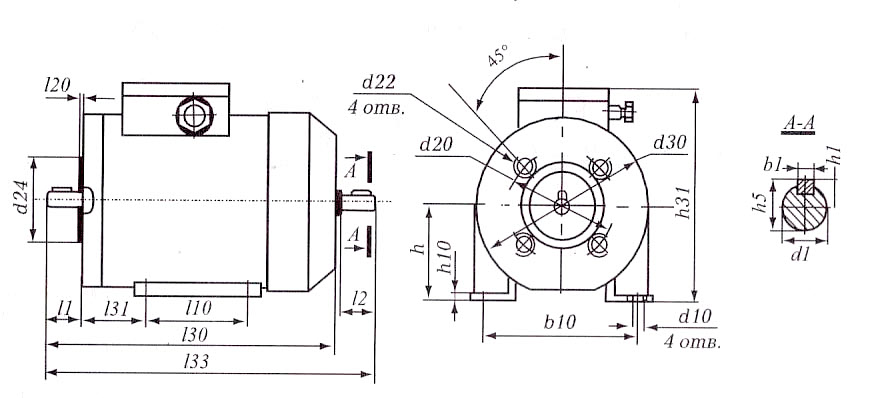
\includegraphics[width=0.8\linewidth]{%
                    img/motor-overall-dimentions}
            }
            \caption{%
                Габаритно-установочные и присоединительные размеры
                двигателя АИР56АУ3
            }
            \label{fig:motor-overall-dimentions}
        \end{figure}
	
        % Габаритные размеры двигателя
        \begin{longtable}{|c|c|c|c|c|c|c|c|}
            \caption{Габаритные размеры двигателя АИР56АУ3
                \label{table:motor-overall-dimentions}}\\
            \hline
            L30 & L33 & d30 & L31 & L1 & L2 & L10 & L20\\
            \hline
            \endfirsthead
            203 & 230 & 80/99 & 141 & 23 & 23 & 71 & 2,5\\
            \hline
        \end{longtable}
        
        % Присоединительные размеры двигателя
        \begin{longtable}{|c|c|c|c|c|c|c|c|c|c|c|c|}
            \caption{Присоединительные размеры двигателя АИР56АУ3
                \label{table:motor-mounting-dimentions}}\\
            \hline
            L31 & d1 & d10 & d20 & d22 & d24 & b1 & b10 & h & h1 & h5 & h10\\
            \hline
            \endfirsthead
            36 & 11 & 5,8 & 85 & М5/М6 & 50/70 & 4 & 90 & 56 & 4 & 12,5 & 7\\
            \hline
        \end{longtable}	

        % Паспортные данные асинхронного двигателя АИР54А4У3
        \begin{longtable}{|c|c|c|c|c|c|c|c|c|c|}
            \caption{Паспортные данные асинхронного двигателя АИР54А4У3
                \label{table:motor-params}}\\
            \hline
            \begin{sideways} Тип двигателя \end{sideways} &
            \begin{sideways} \parbox{6cm}{%
                Номинальная мощность, Вт} \end{sideways} &
            \begin{sideways} \parbox{6cm}{%
                Номинальная  частота вращения, об/мин} \end{sideways} &
            \begin{sideways} \parbox{6cm}{%
                Номинальное напряжение, В} \end{sideways} &
            \begin{sideways} Коэффициент мощности \end{sideways} &
            \begin{sideways} Номинальный ток, А \end{sideways} &
            \begin{sideways} Номинальный момент, Нм \end{sideways} &
            \begin{sideways} \parbox{6cm}{%
                Отношение пускового тока к номинальному} \end{sideways} &
            \begin{sideways} \parbox{6cm}{%
                Отношение максимального момента к номинальному} \end{sideways} &
            \begin{sideways} КПД,\% \end{sideways}\\
            \hline
            \endfirsthead
            АИР56А4У3 & 120 & 1350 & 220 & 0,66 & 0,76 & 0,84 & 5,5 & 2,2 & 63\\
            \hline
        \end{longtable}	

    \subsection{Технические характеристики датчиков перемещения}
        Датчик поворотный дискретный фотоэлектрический ПДФ-5 предназначен
        для преобразования пути (угла поворота) рабочих органов промышленных
        механизмов в число импульсов, а угловой скорости - в частоту следования
        импульсов. 

        Технические характеристики 
        \begin{itemize}
        \item количество выходных каналов - 6. Выходные сигналы (все сигналы
            представлены в прямом и инверсном виде). Две серии импульсов и
            нулевой импульс (один на оборот вала); 
        \item число импульсов в каждой серии на один оборот вала - 600;
        \item Максимальный ток нагрузки каждого канала, мА - 30;
        \item Максимальная частота вращения входного вала - 4000 об/мин;
        \item Номинальное напряжение питания постоянного тока, В - 24;
        \item Номинальное напряжение питания постоянного тока, В - 24;
        \end{itemize}

        Работа выключателя основана на модуляции светового потока,
        направленного от источника излучения через диск с прорезями на
        фотоприемник. При воздействии светового потока на фотоприемник в момент
        прохождения через прозрачный участок диска с выхода выключателя
        снимается сигнал "1". Если световой поток подается на непрозрачный
        участок, и фотоприемник затемнен, на выходе выключателя появляется
        сигнал "0".  
        
        Затем сигнал с фотоприемника усиливается и формируется. После усиления
        по мощности сигнал поступает на разъем, подключаемый к внешней схеме. 

        Датчик (рисунок \ref{fig:encoder}) смонтирован в цилиндрическом литом
        корпусе из алюминиевого сплава, закрытом с двух сторон крышками.
        Подвижный растровый диск укреплен на валу, неподвижный индикаторный
        приклеен к обойме для размещения фотодиодов. Выводы фотодиодов и
        светоизлучателей подпаяны к платам. Элементы электронной схемы
        расположены на трех печатных платах: на двух одинаковых
        усилители-формирователи каналов, на третьей усилитель-формирователь
        нулевого импульса. Цепи выключателя выведены на штепсельный разъем.

        \begin{sidewaysfigure}
            \center{%
                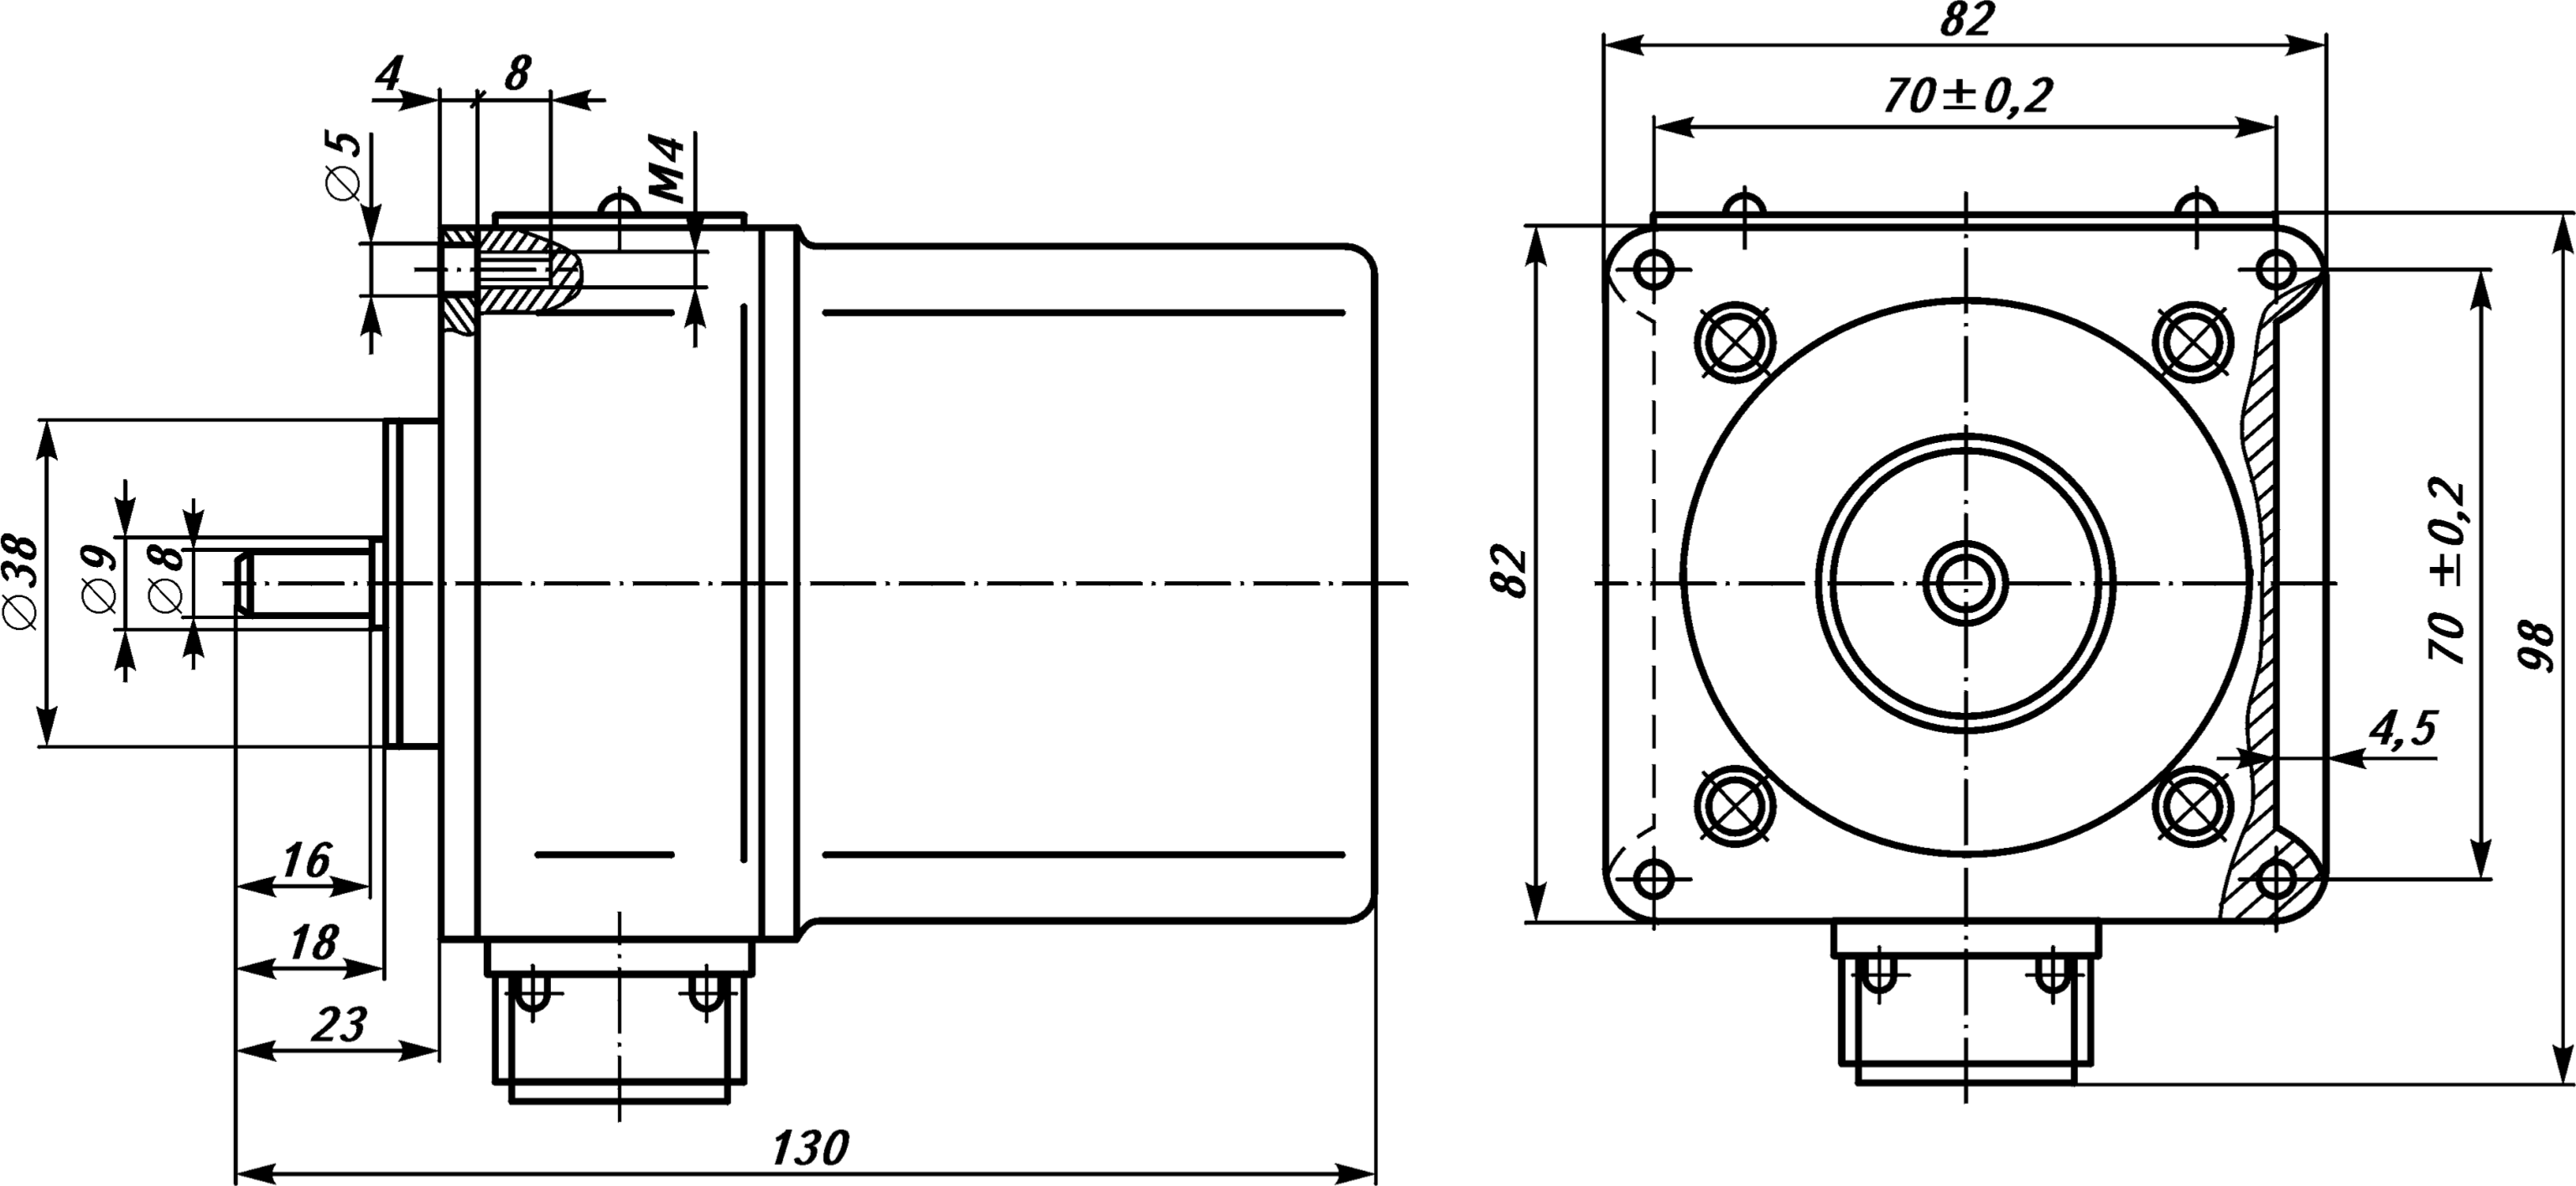
\includegraphics[width=0.8\linewidth]{%
                    img/encoder}
            }
            \caption{%
                Общий вид, габаритные, установочные и присоединительные размеры
                датчика перемещения ПДФ-5
            }
            \label{fig:encoder}
        \end{sidewaysfigure}
        
    \subsection{Электрическая принципиальная схема и описание работы блока
        управления базовой системы}

        Блок управления, схема которого изображена на рисунке
        \ref{fig:mcu-block-schematic} представляет собой МК с набором деталей
        необходимым для его функционирования, а также схемы гальванической
        развязки блока МК с платой драйвера  инвертора, гальванической развязки
        интерфейса датчика скорости и гальванической развязки UART интерфейса
        для связи с ПК.  UART интерфейс обеспечивает соединение с ПК для
        управления и контроля работы электропривода, а также отладки внутренней
        программы МК.
            
        \begin{sidewaysfigure}
            \center{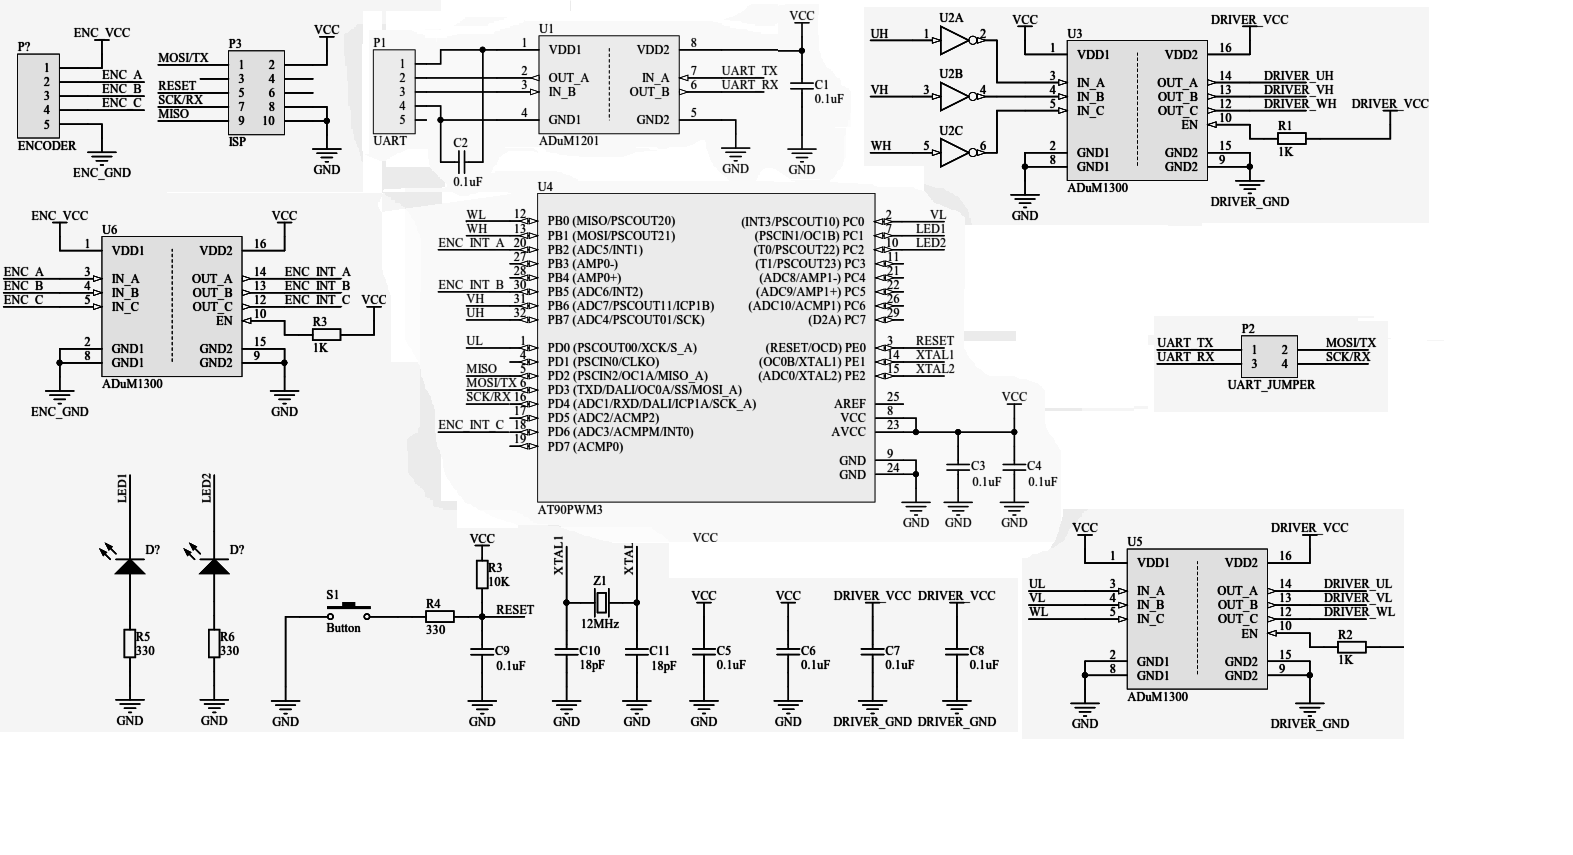
\includegraphics[width=0.8\linewidth]{%
                img/mcu-block-schematic}}
            \caption{Принципиальная электрическая схема блока управления на
                основе МК AT90PWM3}
            \label{fig:mcu-block-schematic}
        \end{sidewaysfigure}
        
        Основой блока управления является микроконтроллер AT90PWM3, структурная
        схема которого показана на рисунке \ref{fig:at90pwm3}.
        
        AT90PWM3 представляет собой экономичный однокристальный
        микроконтроллер, c производительностью до 16 миллионов инструкций в
        секунду. Он предназначен для выполнения функций управления в
        понижающих/повышающих преобразователях постоянного напряжения,
        синхронными электрическими машинами на основе постоянных магнитов,
        трехфазными асинхронными электродвигателями и бесколлекторными
        электродвигателями постоянного тока. 

        \begin{figure}[h!]
            \center{%
                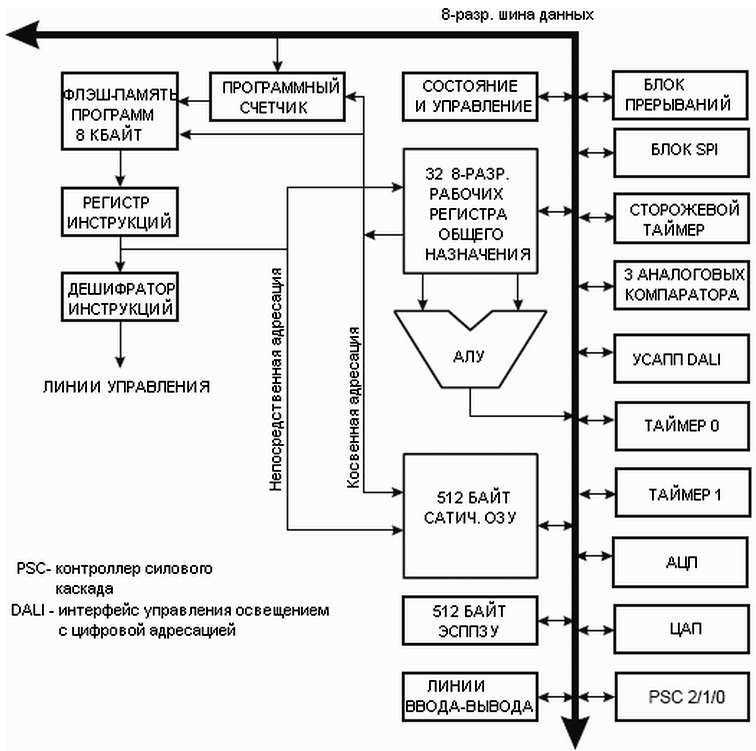
\includegraphics[width=0.8\linewidth]{%
                    img/at90pwm3}
            }
            \caption{Структурная схема микроконтроллера AT90PWM3}
            \label{fig:at90pwm3}
        \end{figure}
        
        Особенностью данного микроконтроллера является наличие блока PSC (Power
        Stage Controller) позволяющего генерировать широтно-модулированный
        сигнал управления тремя полумостами силовых транзисторов. 
        
        Элемент U2 – 74HC04 представляет собой логический инвертор,
        инвертирующий уровни на выходах UH, WH и VH микроконтроллера, так как
        применённая в данной работе ревизия чипа микроконтроллера AT90PWM3
        имеет недоработку состоящую в отсутствии  сдвига фаз на 180 градусов
        между выходными сигналами МК управляющими верхними и нижними ключами
        инвертора.
        
        Микросхемы гальванической развязки U1, U3, U5 и U6 обеспечивают полную
        гальваническую развязку платы блока управления с внешними устройствами,
        тем самым обеспечивают безопасность микроконтроллера в случае
        возникновения аварийной ситуации во внешних цепях, а также в цепях
        связи платы управления с ПК. Микросхема U1 – ADUM1201, представляет
        собой двухканальный двунаправленный цифровой изолятор. U3, U5, U6 –
        ADUM1300 трёхканальные однонаправленные цифровые изоляторы.
        
        Блок микроконтроллера обеспечивает функции плавного пуска, останова,
        реверса электродвигателя, регулировку частоты вращения асинхронного
        электродвигателя с отображением графика её изменения на мониторе
        персонального компьютера.
        
        Внутренняя программа МК реализует разомкнутую систему скалярного
        управления асинхронной машиной переменного тока по принципу постоянства
        отношения $V/f$. Алгоритм работы программы представлен на рисунке
        \ref{fig:old-algorithm}

        \begin{figure}
            \center{%
                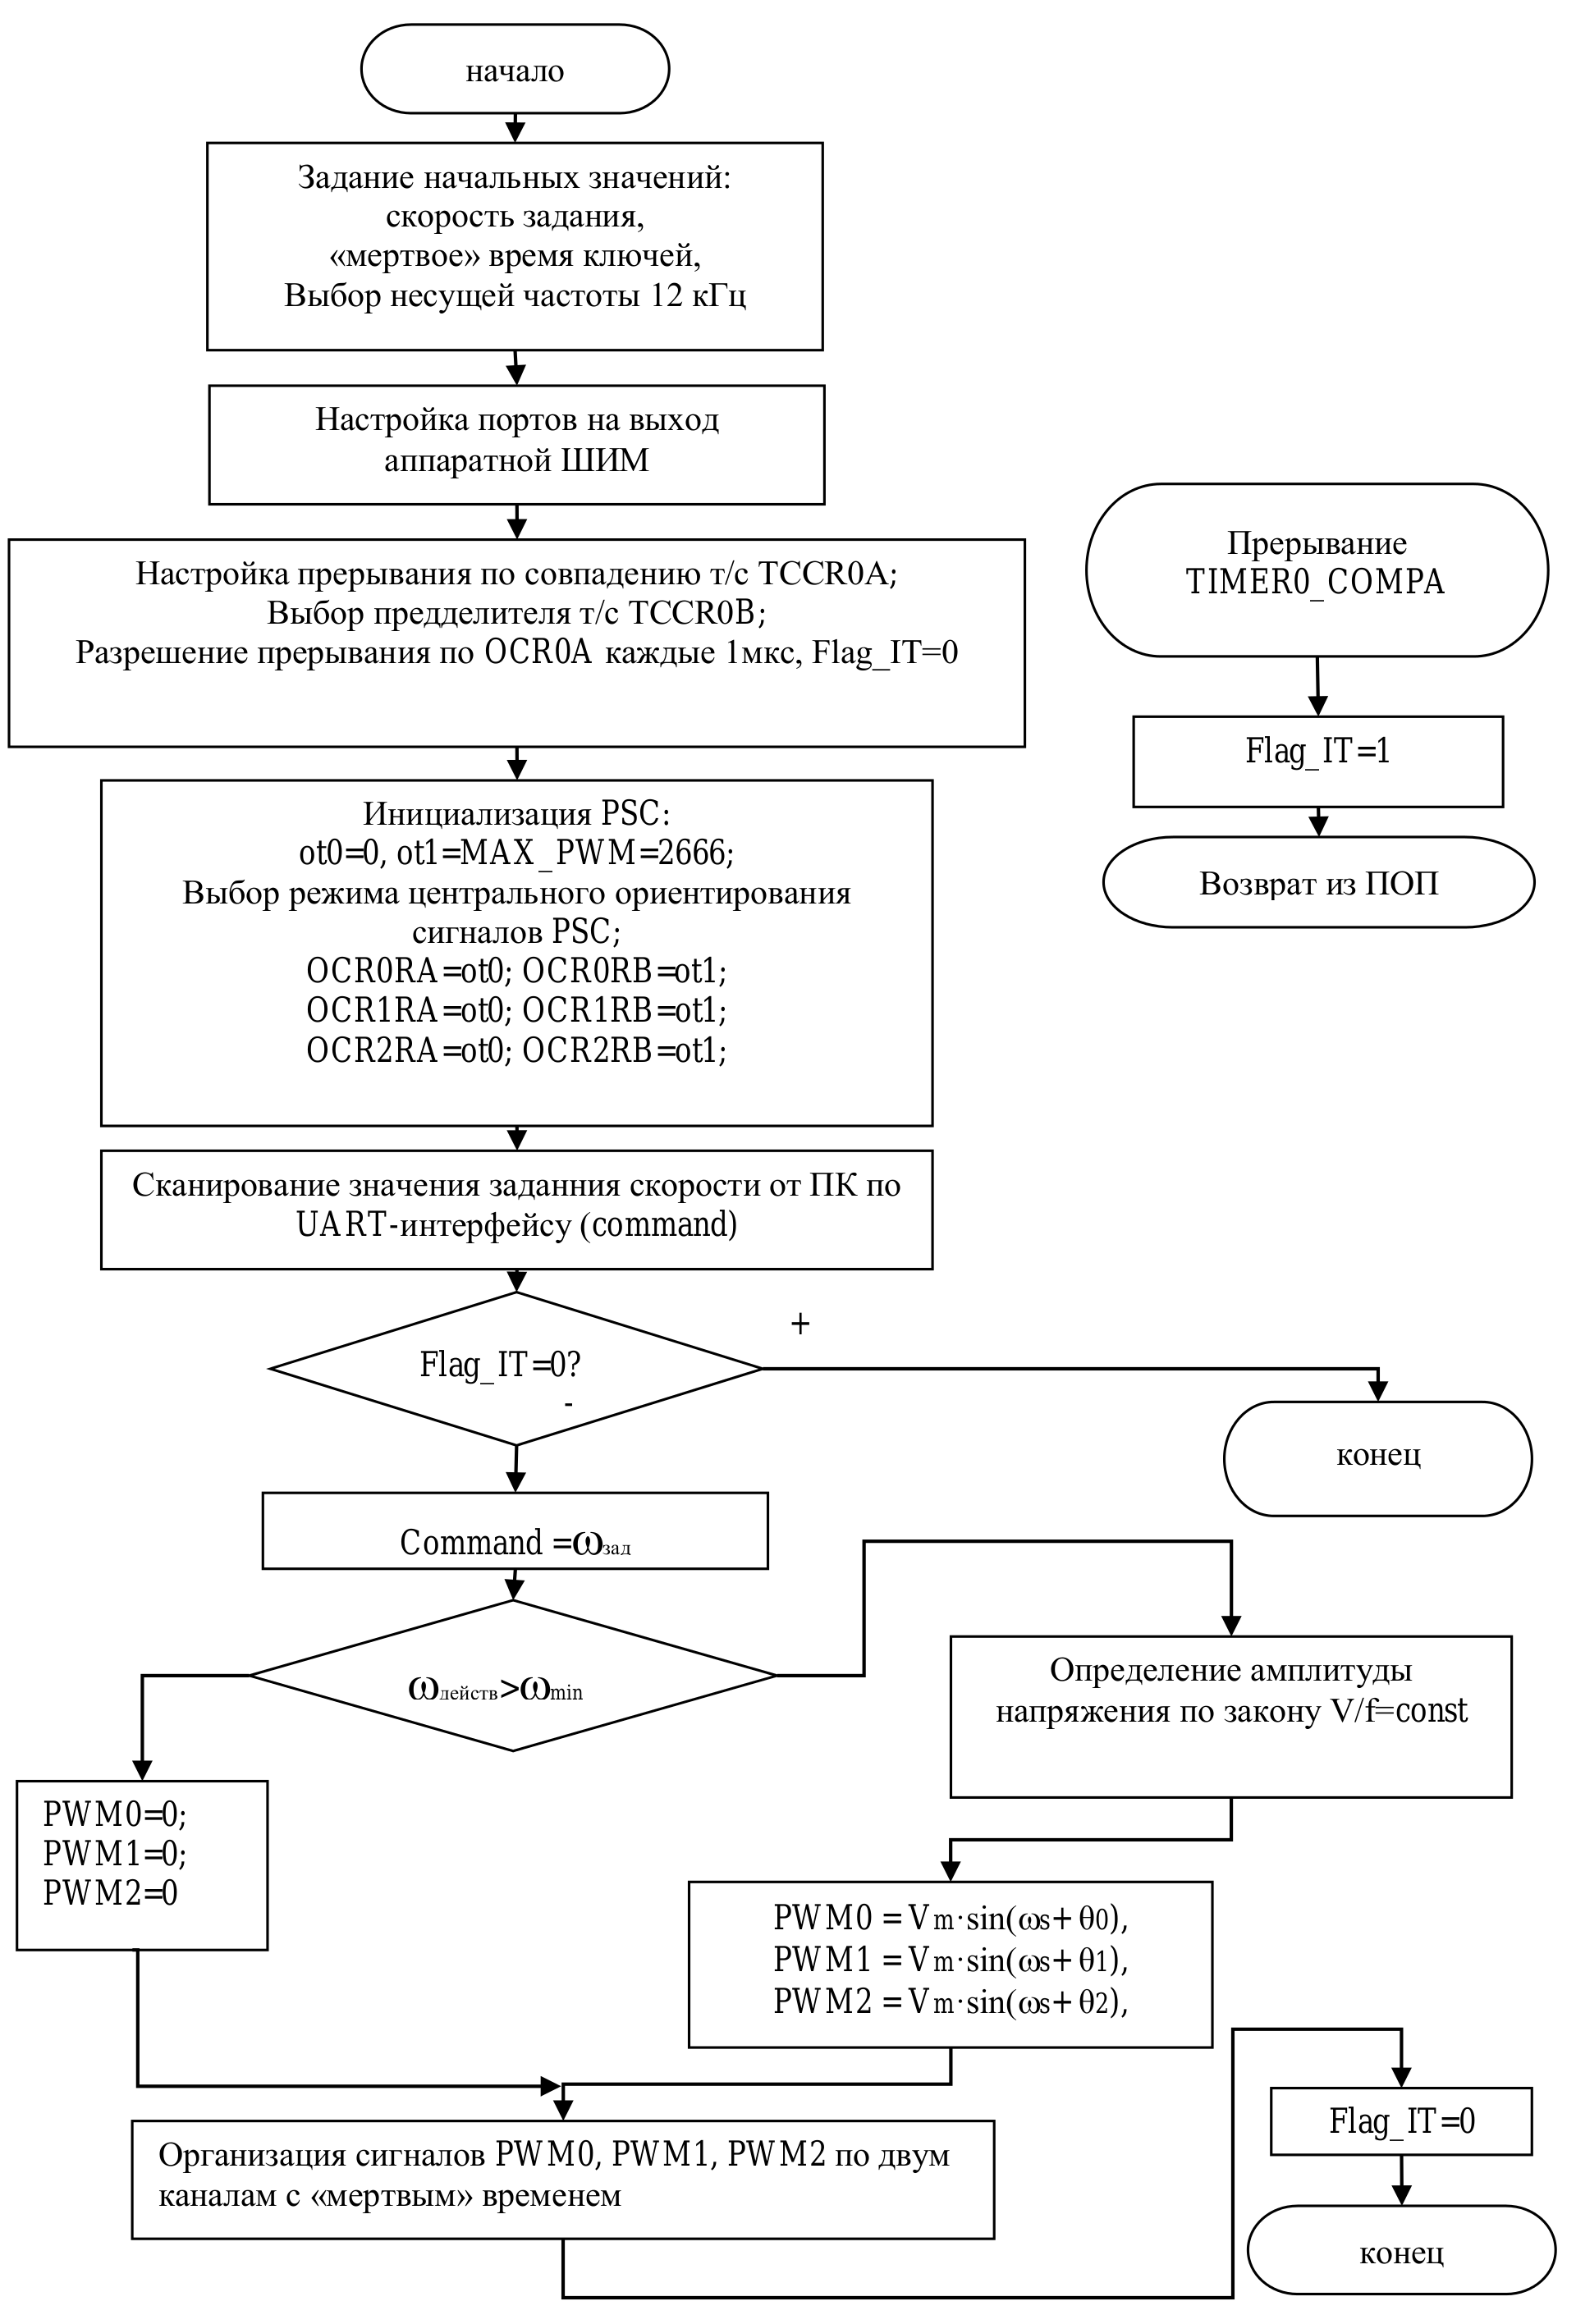
\includegraphics[width=0.9\linewidth]{%
                    img/old-algorithm}
            }
            \caption{Алгоритм работы программы МК базовой системы}
            \label{fig:old-algorithm}
        \end{figure}


    \subsection{Электрическая принципиальная схема и описание работы блока
        инвертора напряжения}

        Принципиальная схема инвертора представлена на рисунке
        \ref{fig:power-block-schematic}. В качестве ключевых транзисторов T1-T6
        выбраны полевые транзисторы типа IRF740.
        
        \begin{sidewaysfigure}
            \center{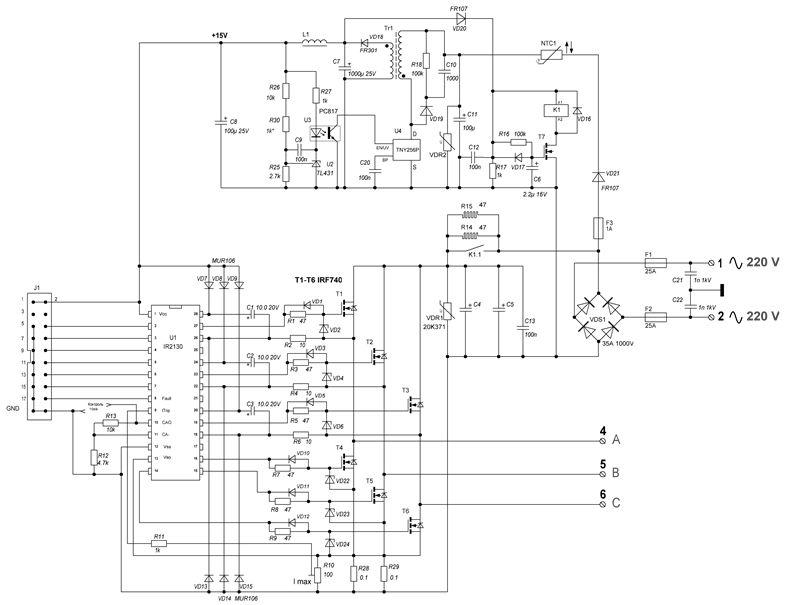
\includegraphics[width=0.8\linewidth]{%
                img/power-block-schematic}}
            \caption{Принципиальная электрическая схема АИН на основе драйвера
                IR2130}
            \label{fig:power-block-schematic}
        \end{sidewaysfigure}
        
        Для непосредственного управления силовыми ключами использована
        специализированная ИМС драйвер трёхфазного моста IR2130, структурная
        схема которой представлена на рисунке \ref{fig:ir2130}. Она
        обеспечивает согласование выходных сигналов блока микроконтроллера с
        силовой частью, а также обеспечивает контроль мёртвого времени силовых
        ключей и защиту выходного каскада от перегрузок по току.

        \begin{figure}[h!]
            \center{%
                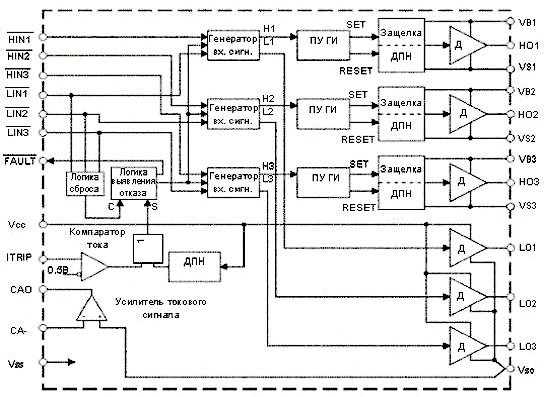
\includegraphics[width=0.8\linewidth]{%
                    img/ir2130}
            }
            \caption{Структурная схема драйвера трехфазного моста IR2130}
            \label{fig:ir2130}
        \end{figure}

        На схеме элементы С21, С22, С11, С12, С14 и VDS1 образуют входной
        сетевой фильтр и входной выпрямитель. Резисторы  R26 и R27 вместе с
        реле K1 и устройством задержки включения на транзисторе Т7 представляют
        собой схему «мягкого» включения инвертора в сеть, необходимую для
        ограничения тока зарядки конденсаторов С11 и С12 и подачи полного
        напряжения питания на транзисторы Т1-Т6 только после полного включения
        ИМС IR2130 и прекращения всех переходных процессов в инверторе, что
        увеличивает надёжность и долговечность работы устройства. 
        
        На микросхеме U4 –TNY256p собран импульсный блок питания,
        обеспечивающий стабилизированное выходное напряжение 15В для питания
        драйвера IR2130.  Микросхема TNY256 представляет собой
        специализированный ШИМ контроллер, предназначенный для создания
        импульсных блоков питания небольшой мощности с минимальным количеством
        навесных компонентов.
        
        Плата автономного инвертора напряжения установлена в корпус от
        импульсного блока питания ПК. Силовые транзисторы выходного каскада
        прикреплены к теплоотводу через изоляционные термопроводящие прокладки.
